% Appendix
\chapter{Appendix}


\seb{change appendix name or way it is displayed. I want to have just 1 appendix}

\begin{figure}[H]
  \centering
  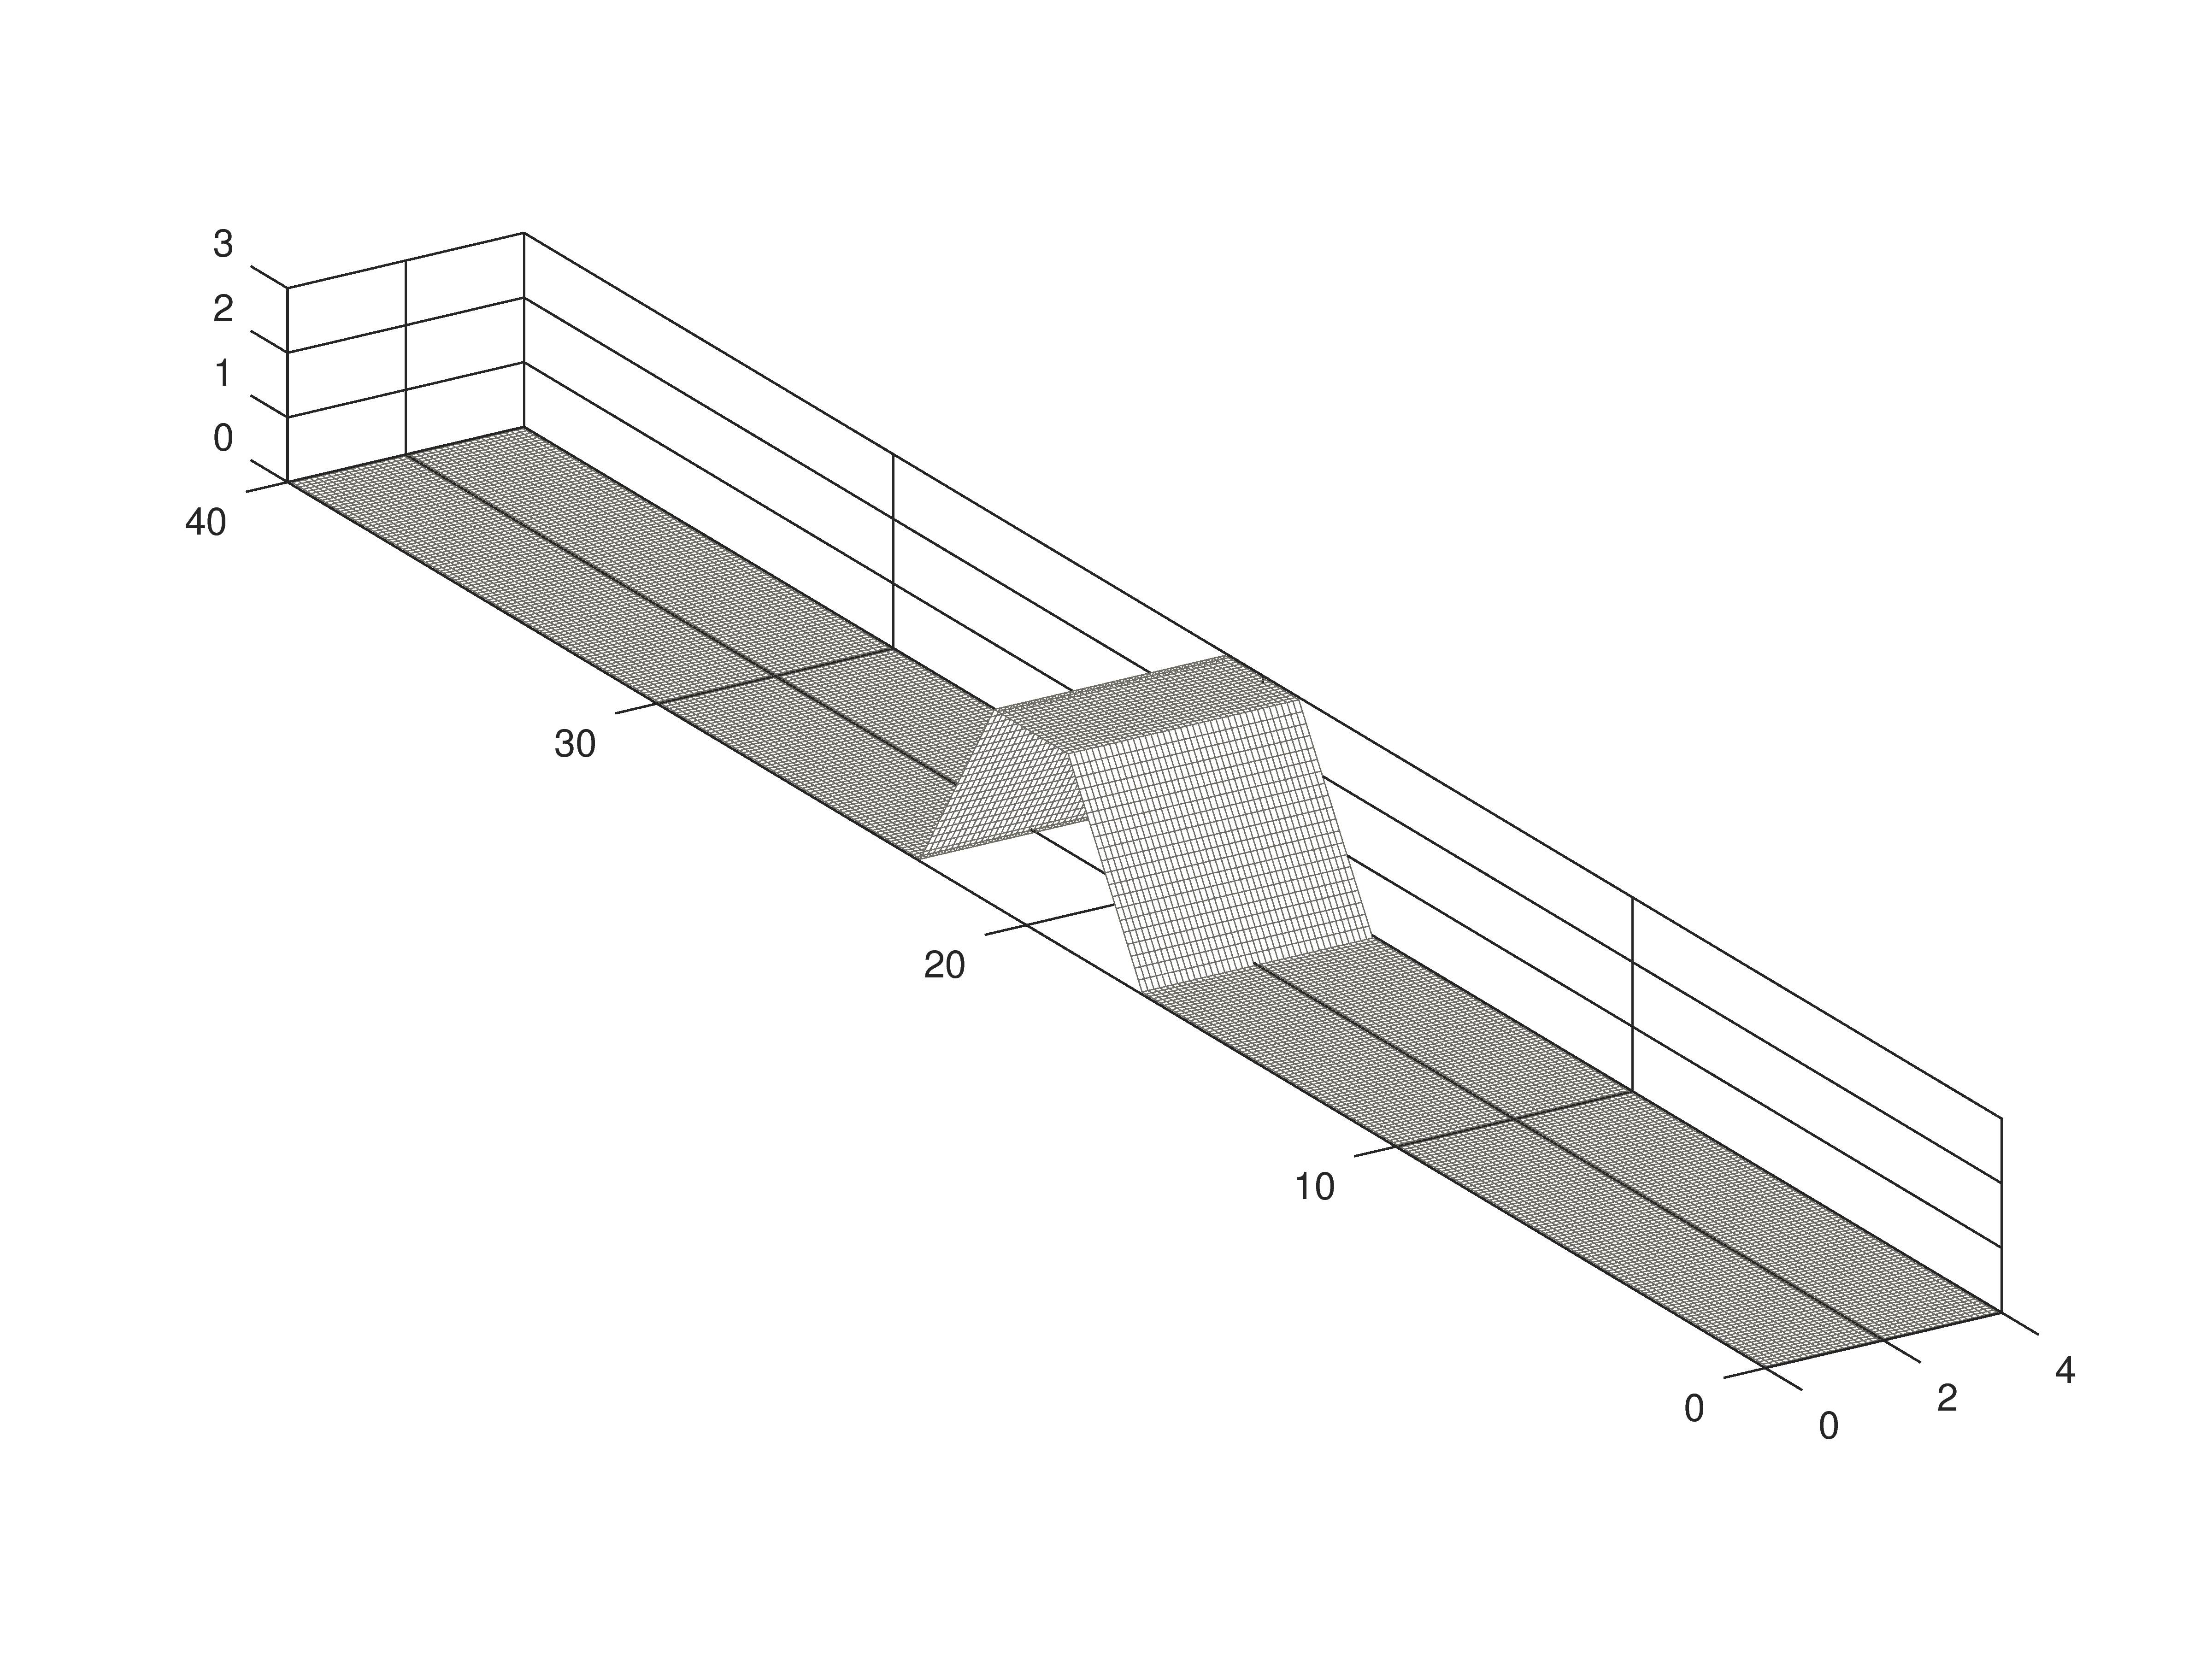
\includegraphics[width=0.8\textwidth]{Figures/channel.png}
  \caption{Topography of the channel used for \emph{case study 1}. The channel presents no walls because "wall boundary conditions" were chosen in \textit{FullSWOF\_2D} for the two lateral boundaries.}
  \label{fig:channel}
\end{figure}
\seb{does it make sense to put this figure?}


\begin{figure}[H]
  \centering
  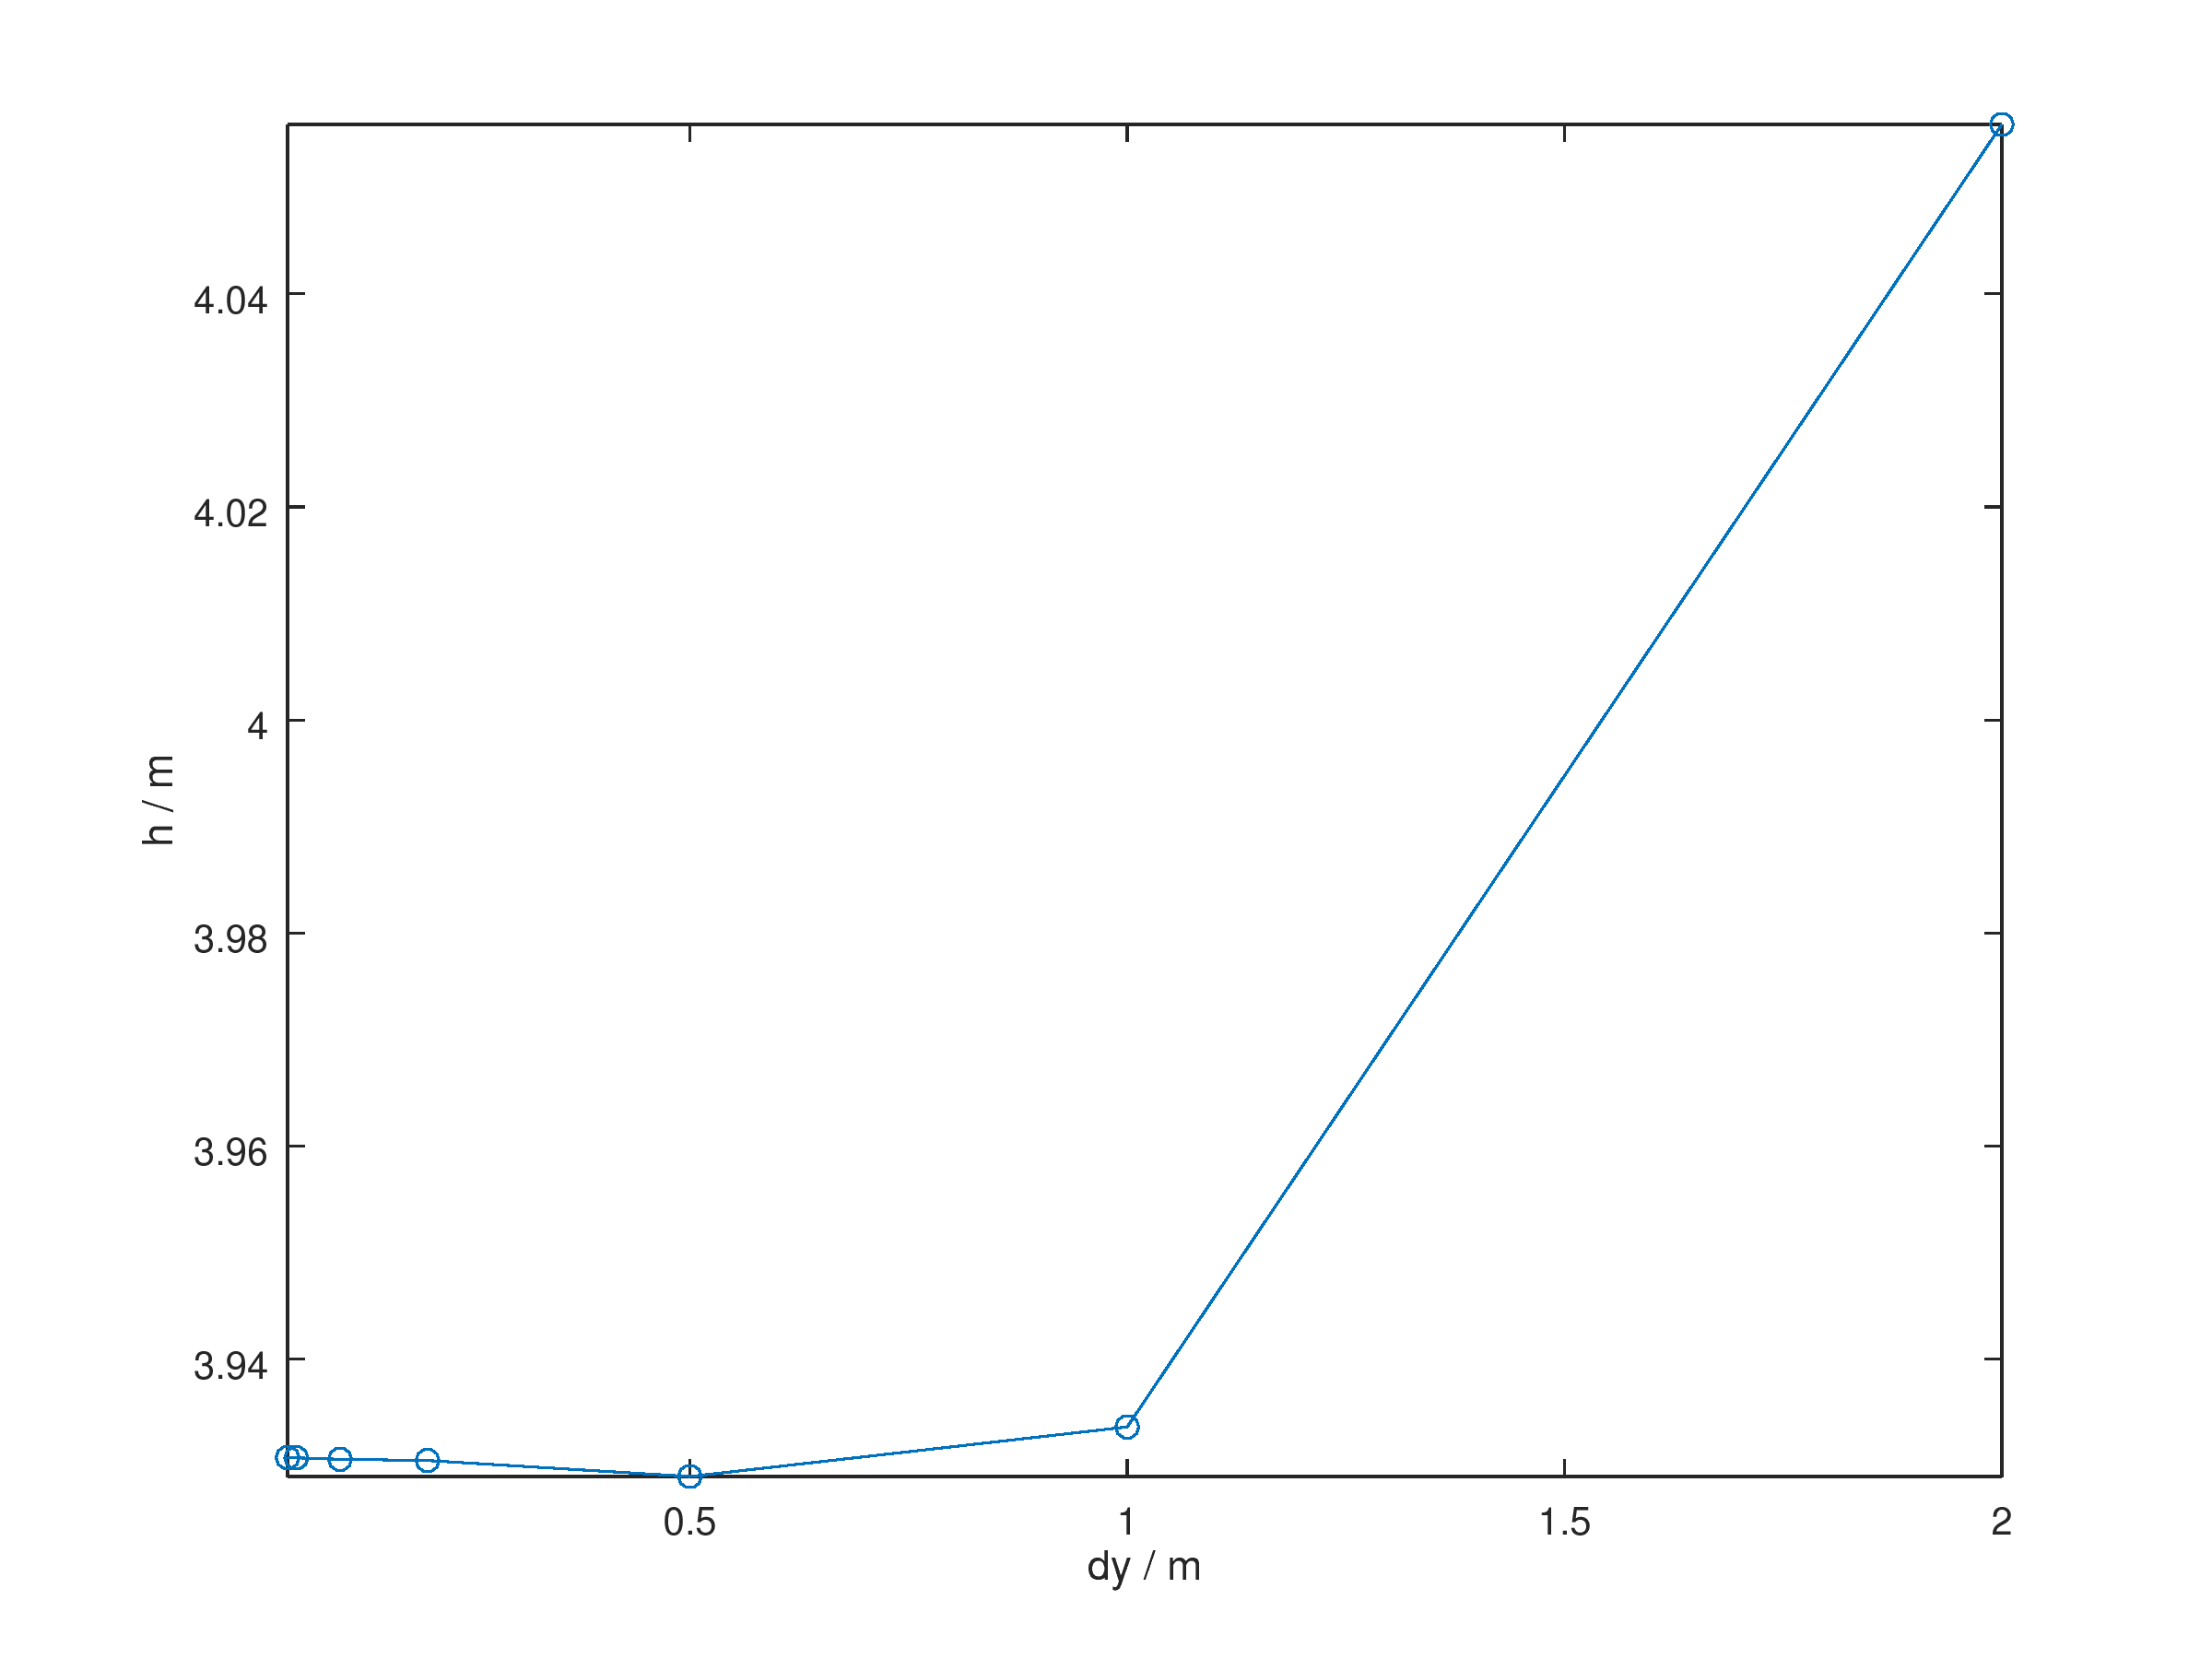
\includegraphics[width=0.7\textwidth]{Figures/convergence_center.png}
  \caption{Measured free surface height at the weir midpoint as a function of the grid resolution used.}
  \label{fig:convergence_center}
\end{figure}


\begin{table}[H]
  \centering
  \caption{Dataset used for computing the model error.}
  \label{tab:dataset_error}
  \begin{adjustbox}{max width=\textwidth}
    \begin{tabular}{lrrrrrrrrrrrrrr}
      \toprule
      $\bm{h_w}\,/\si{\m}$             & 0.00 & 0.50 & 0.55 & 0.61 & 0.66 & 0.80 & 0.89 & 0.93 & 1.05 & 1.08 & 1.20 & 1.16 & 1.27 & 1.30\\
      $\bm{Q}$\,/\si{\cubic\m\per\s}   & 0.00 & 2.16 & 2.58 & 2.99 & 3.40 & 4.64 & 5.46 & 5.88 & 7.11 & 7.53 & 8.76 & 8.35 & 9.59 & 10.00\\
      \bottomrule
    \end{tabular}}
  \end{adjustbox}
\end{table}


\begin{figure}[h]
  \centering
  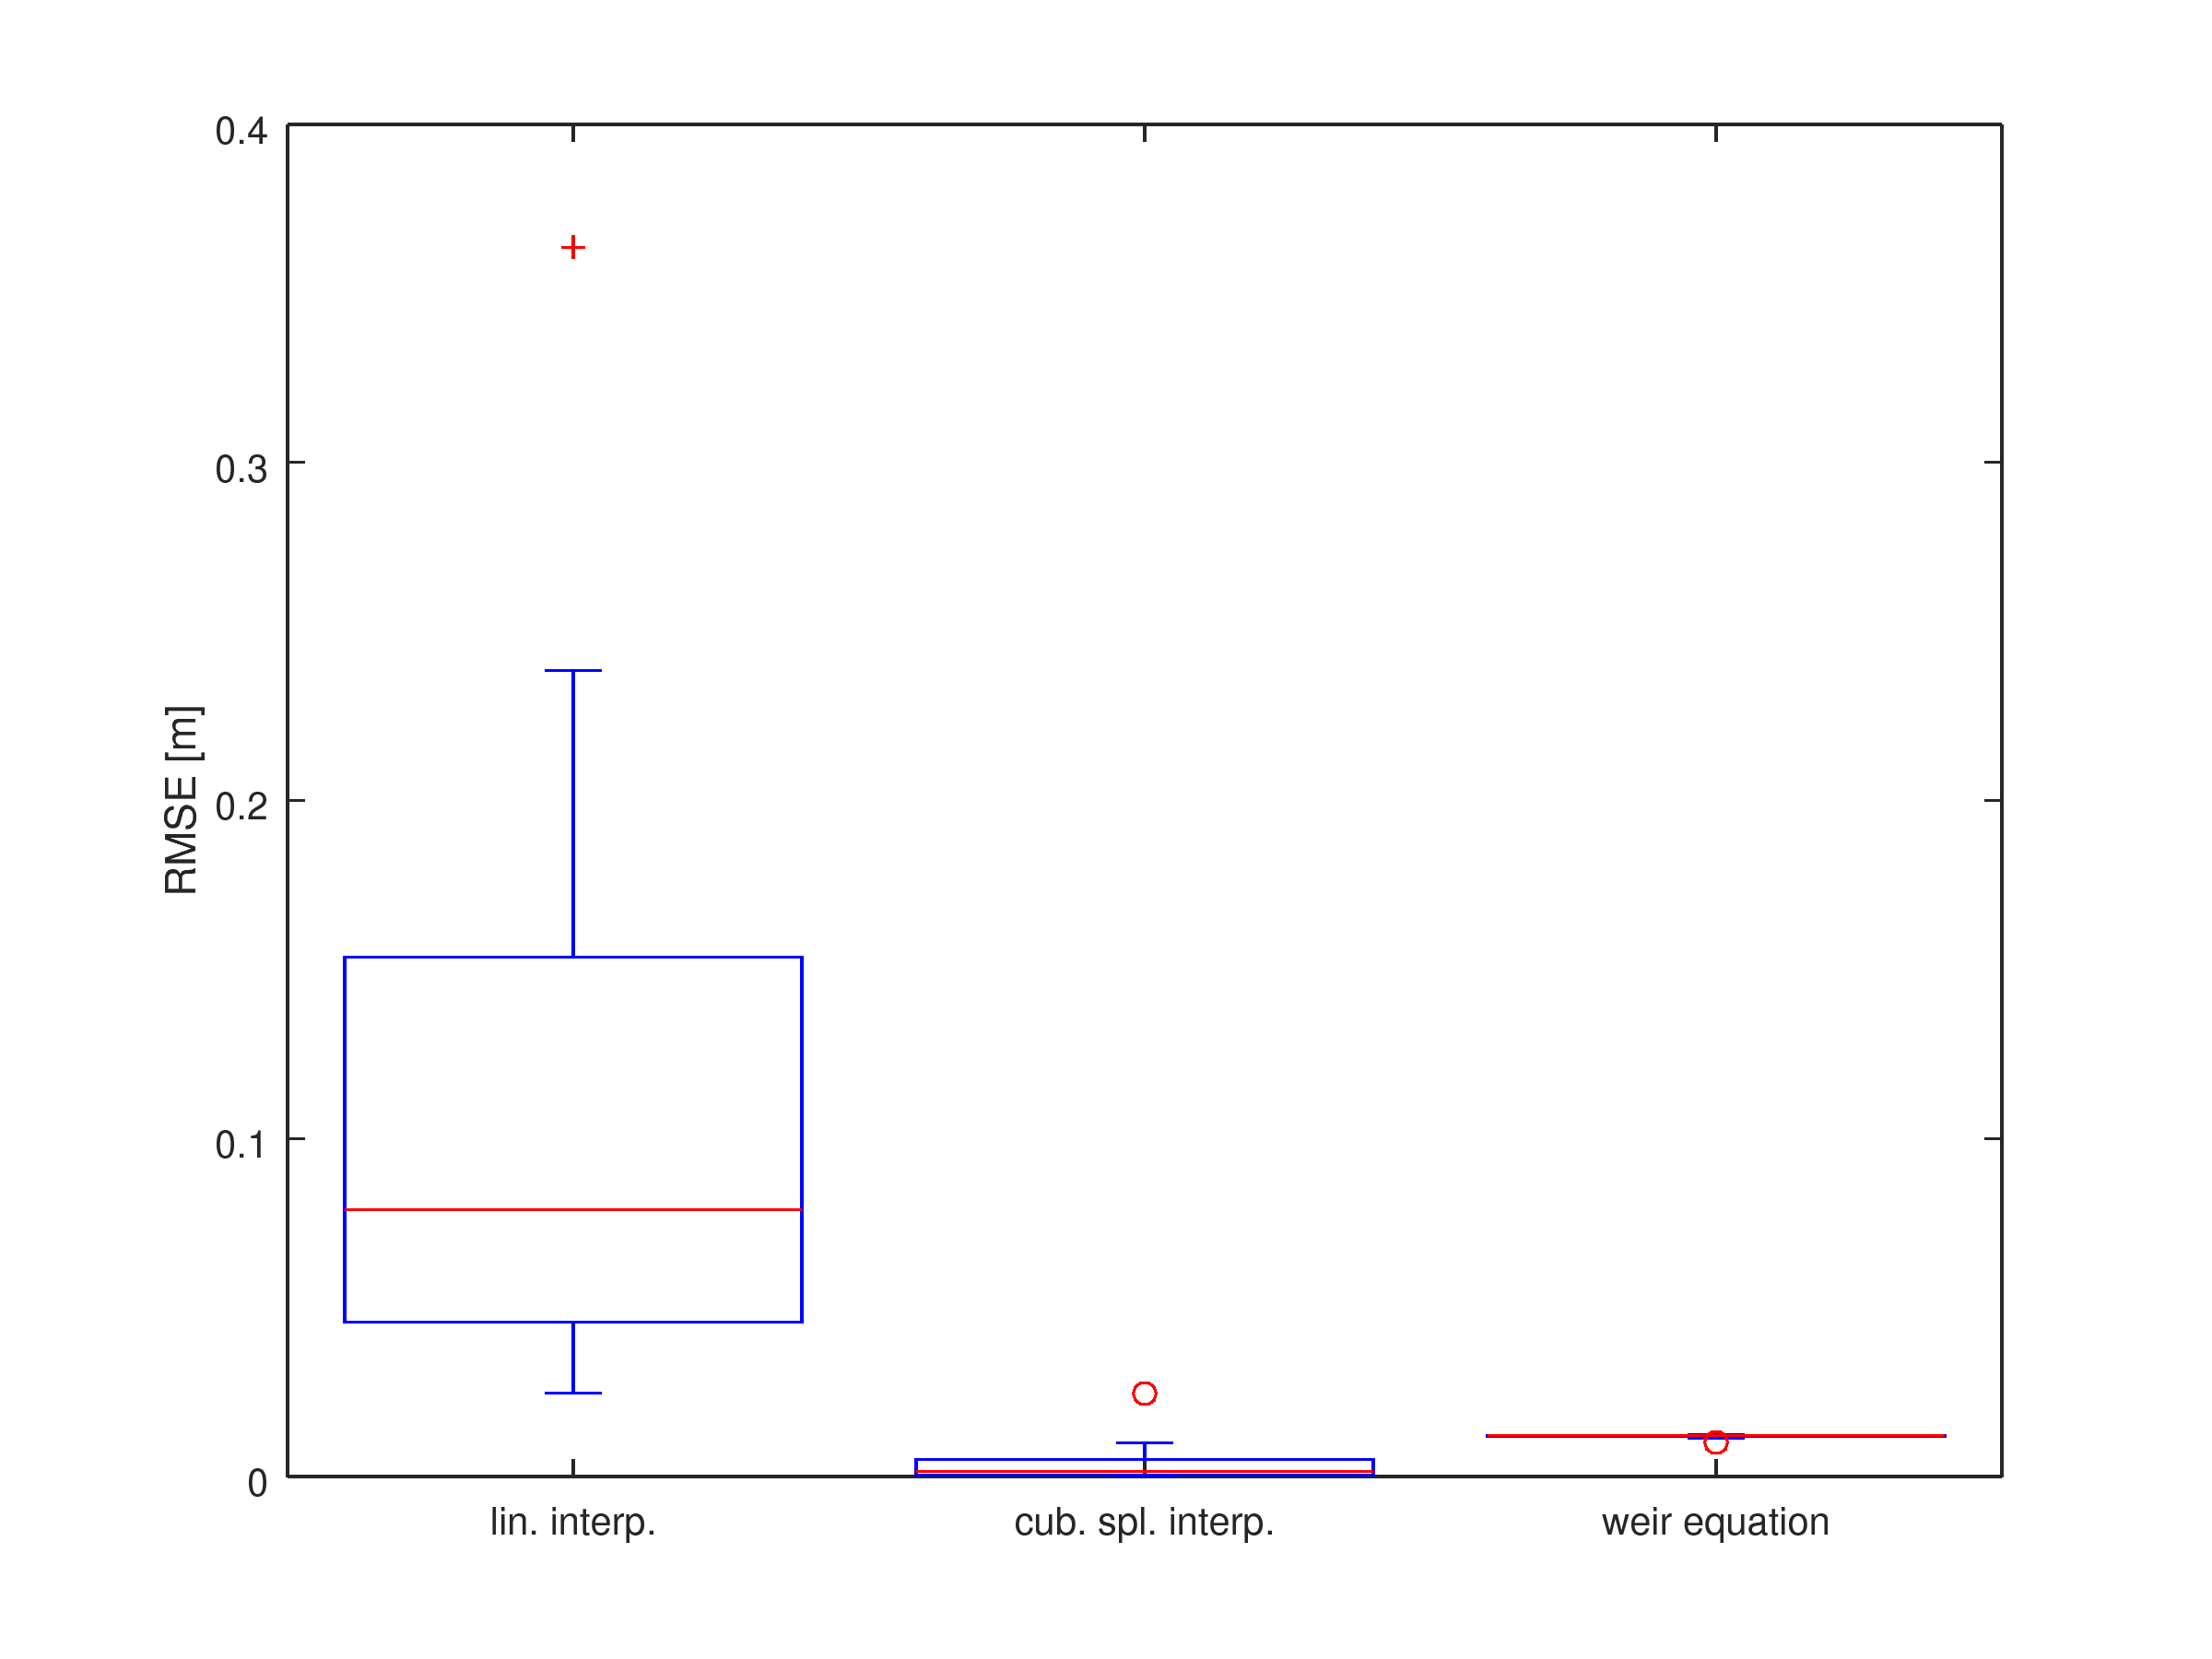
\includegraphics[width=0.7\textwidth]{Figures/boxplot_models.png}
  \caption{Box plot summarizing the performance of the three models by using $[\numrange{4}{13}]$ \# of points. The red line represent the median RMSE. The box is given by the \nth{1} and \nth{3} quartile. Whiskers are drawn at $1.5 \times IQR$. Points between $1.5 \times IQR$ and $3 \times IQR$ are marked with 'o', while '+' indicates points beyond this range \autocite{eaton_gnu_2016}.}
  \label{fig:boxplot_models}
\end{figure}


\begin{table}[H]
  \centering
  \caption{Emulator training dataset}
  \label{tab:training_dataset}
  \begin{tabular}{lccc}
    \toprule
     & \textbf{1} & \textbf{2} & \textbf{3}\\
    \midrule
    $\bm{I}$ \textbf{[\si{\milli\meter\per\hour}]} & val & val & val \\
    $\bm{\theta_i}$ \textbf{[--]} & val & val & val \\
    \bottomrule
  \end{tabular}
\end{table}


\begin{table}[H]
  \centering
  \caption{Emulator test dataset}
  \label{tab:test_dataset}
  \begin{tabular}{lccc}
    \toprule
     & \textbf{1} & \textbf{2} & \textbf{3}\\
    \midrule
    $\bm{I}$ \textbf{[\si{\milli\meter\per\hour}]} & val & val & val \\
    $\bm{\theta_i}$ \textbf{[--]} & val & val & val \\
    \bottomrule
  \end{tabular}
\end{table}


\begin{table}[H]
  \centering
  \caption{Emulator validation dataset}
  \label{tab:validation_dataset}
  \begin{tabular}{lccc}
    \toprule
     & \textbf{1} & \textbf{2} & \textbf{3}\\
    \midrule
    $\bm{I}$ \textbf{[\si{\milli\meter\per\hour}]} & val & val & val \\
    $\bm{\theta_i}$ \textbf{[--]} & val & val & val \\
    \bottomrule
  \end{tabular}
\end{table}


\begin{table}[H]
  \centering
  \caption{Emulator performance on every validation point}
  \label{tab:validation_performance}
  \begin{tabular}{lccc}
    \toprule
     & \textbf{1} & \textbf{2} & \textbf{3}\\
    \midrule
    \textbf{simulated} $\bm{t_!}$ & val & val & val \\
    \textbf{emulated} $\bm{t_!}$ & val & val & val \\
    \bottomrule
  \end{tabular}
\end{table}
